\apendice{Documentación de usuario}

\section{Introducción}
En esta sección, se explica al usuario qué necesita para poder utilizar la aplicación, cómo se instalaría y un manual de usuario para enseñarle cómo funciona.

\section{Requisitos de usuarios} \label{requisitos}
Los requisitos necesarios para poder utilizar la aplicación web son:

\begin{itemize}
	\item Tener un navegador que soporte HTML5, como Google Chrome o Microsoft Edge.
	\item Tener conexión a Internet.
\end{itemize}

Además, dado que es necesario estar dado de alta para utilizar la aplicación, se han preparado unos usuarios específicos para poder realizar pruebas en la aplicación desde un usuario con privilegios y otro sin privilegios:

\begin{itemize}
	\item \underline{Administrador:} 
	\begin{itemize}
		\item \textbf{Nombre de usuario:} admin.
		\item \textbf{Contraseña:} 1234.
	\end{itemize}
	\item \underline{Usuario:}
	\begin{itemize}
		\item \textbf{Nombre de usuario:} usuario.
		\item \textbf{Contraseña:} 1234.
	\end{itemize}
\end{itemize}

\section{Instalación}
Al tratarse de una aplicación web, no necesita nada más allá de un navegador web que soporte HTML5.

\section{Manual del usuario}
En esta sección se explica cómo utilizar la aplicación web.

\subsection{Inicio de sesión}
Nada más acceder a la aplicación web, aparecerá la pantalla de inicio de sesión que representa la figura \ref{fig:inicio_sesion_E}. Para acceder a ella, es necesario estar previamente dado de alta. Los usuarios indicados en el punto \ref{requisitos} pueden ser utilizados para acceder a la aplicación.

En caso de no escribir correctamente el usuario, aparecerá un mensaje indicando que el usuario es incorrecto, como se aprecia en la figura \ref{fig:usuario_no_encontrado_E}. Si la contraseña es incorrecta, aparecerá otro mensaje indicando que el error en el inicio de sesión ha sido la contraseña, tal y como se muestra en la figura \ref{fig:clave_incorrecta_E}, pero que el usuario es correcto.

Dependiendo de si se trata de un usuario con o sin privilegios, aparecerán unas opciones u otras.

\begin{figure}[ht]
	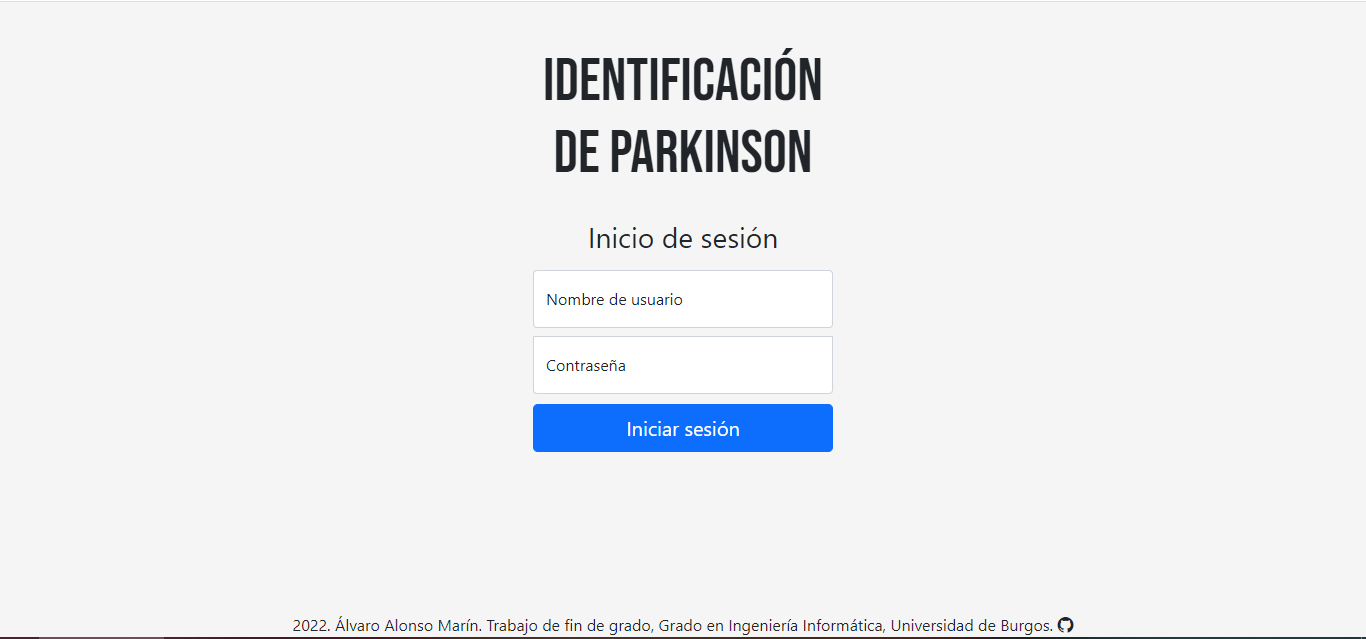
\includegraphics[width=1\textwidth]{inicio_sesion_E}
	\caption{Pantalla del inicio sesión de la aplicación web.}
	\label{fig:inicio_sesion_E}
\end{figure}

\begin{figure}[ht]
	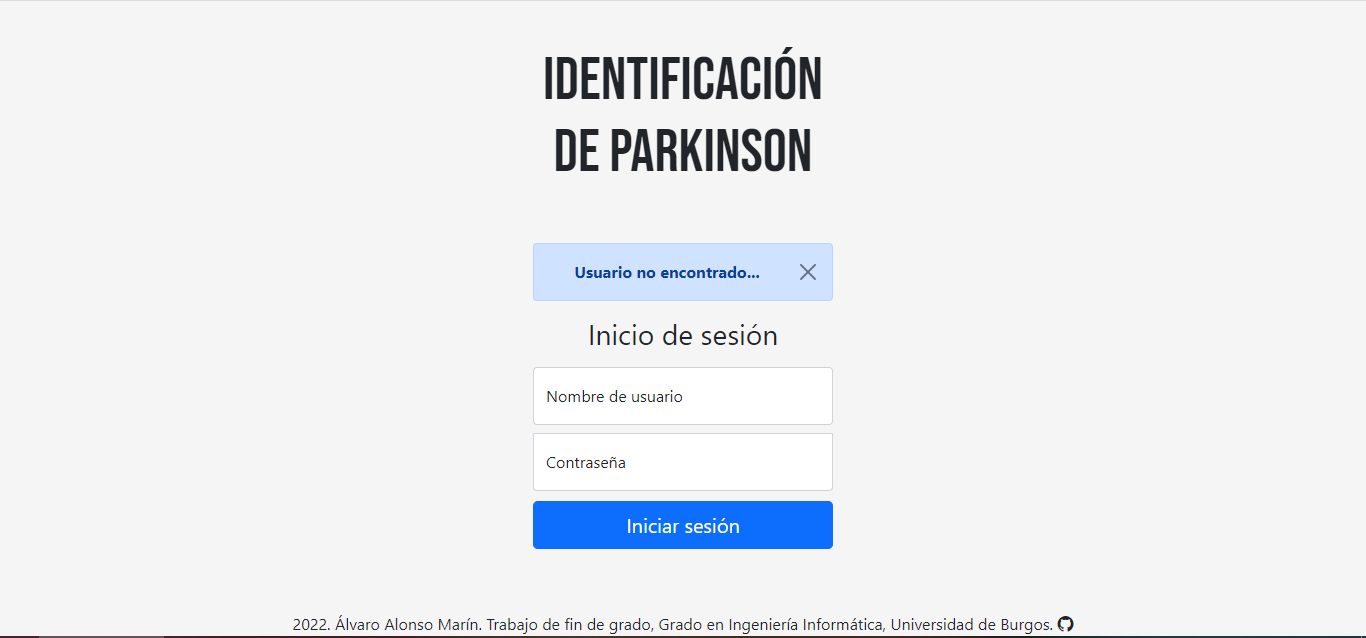
\includegraphics[width=1\textwidth]{usuario_no_encontrado}
	\caption{Pantalla del inicio sesión con el error de usuario no encontrado.}
	\label{fig:usuario_no_encontrado_E}
\end{figure}

\begin{figure}[ht]
	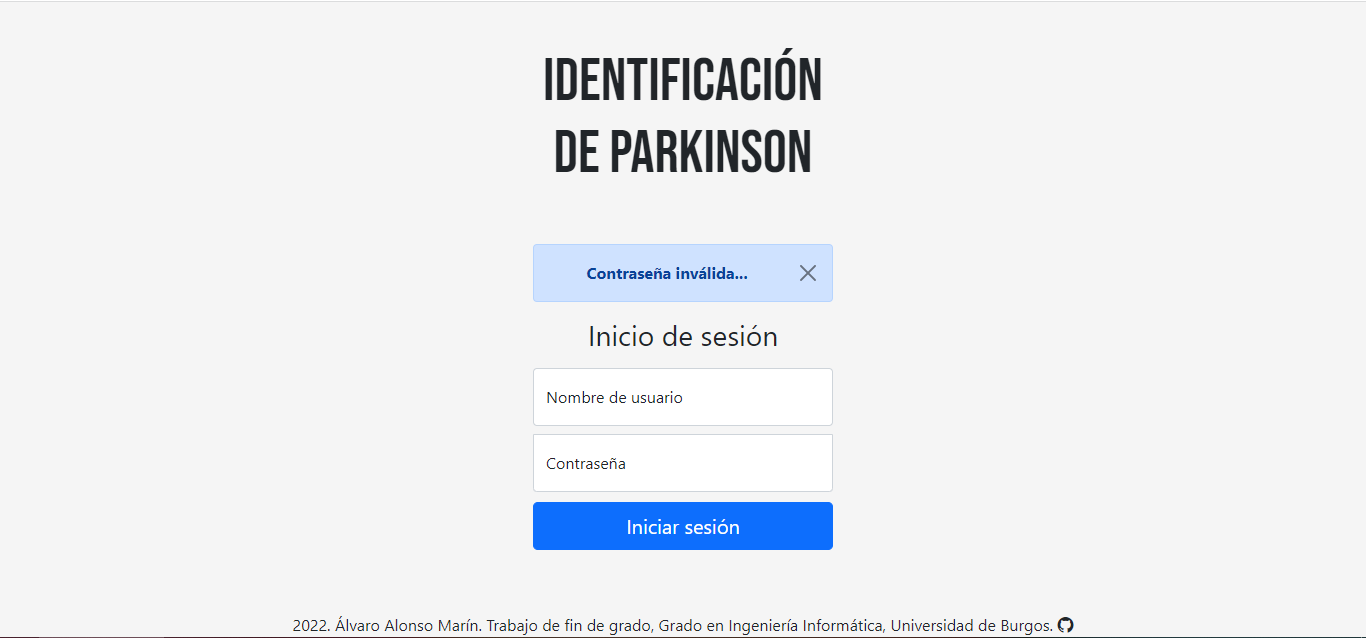
\includegraphics[width=1\textwidth]{clave_incorrecta}
	\caption{Pantalla del inicio sesión con el error de contraseña inválida.}
	\label{fig:clave_incorrecta_E}
\end{figure}

\subsection{Pantalla principal}

\subsubsection{Usuario administrador}
En caso de haber accedido con el usuario administrador, se podrán realizar más operaciones. En esta pantalla se podrá seleccionar el vídeo o arrastrarlo para realizar la predicción, además de seleccionar la mano y el sexo, tal y como se muestra en la figura \ref{fig:pantalla_principal_admin_E}.

\begin{figure}[ht]
	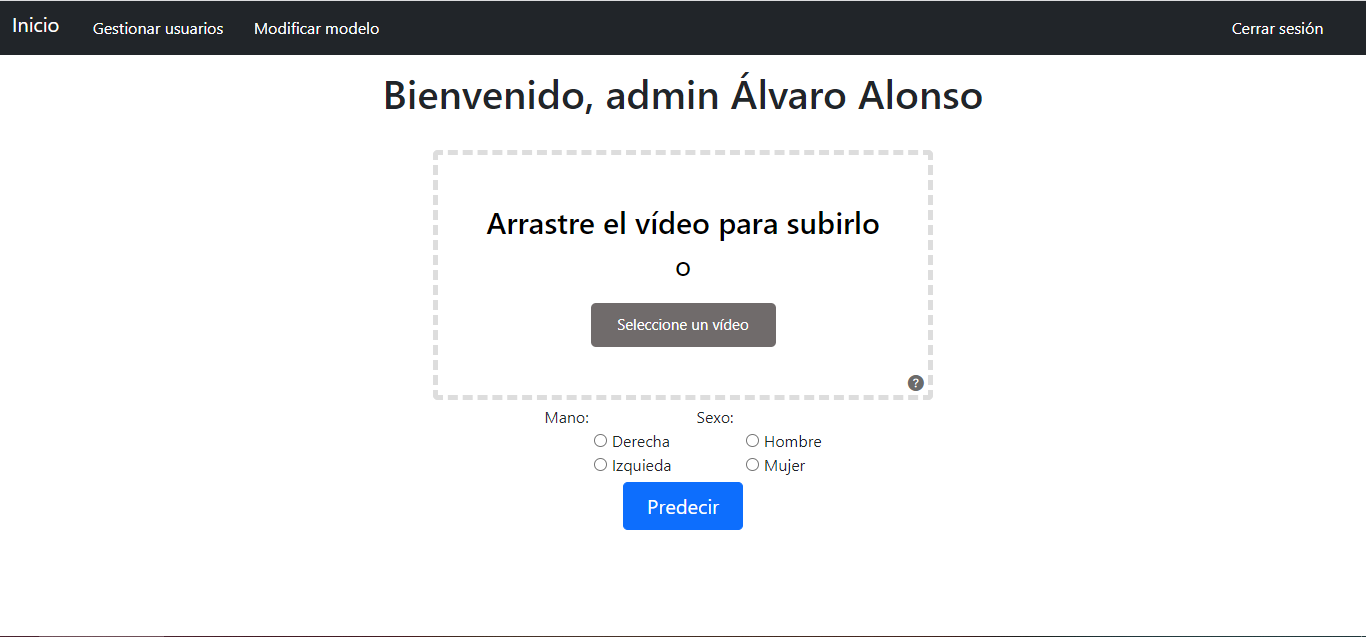
\includegraphics[width=1\textwidth]{pantalla_principal_admin_E}
	\caption{Pantalla principal del administrador para realizar la predicción.}
	\label{fig:pantalla_principal_admin_E}
\end{figure}
